\documentclass{article}


% \usepackage{PRIMEarxiv}
\usepackage[margin=1.5in]{geometry}
\usepackage[utf8]{inputenc} % allow utf-8 input
\usepackage[T1]{fontenc}    % use 8-bit T1 fonts
\usepackage{hyperref}       % hyperlinks
\usepackage{url}            % simple URL typesetting
\usepackage{booktabs}       % professional-quality tables
\usepackage{amsfonts}       % blackboard math symbols
\usepackage{nicefrac}       % compact symbols for 1/2, etc.
\usepackage{microtype}      % microtypography
\usepackage{lipsum}
\usepackage{amsmath}
\usepackage{amsthm}
\usepackage{mathtools}
\usepackage{fancyhdr}       % header
\usepackage{graphicx}       % graphics
\graphicspath{{media/}}     % organize your images and other figures under media/ folder
\usepackage{amssymb}
\usepackage{xcolor}
\usepackage{mwe}
\usepackage{subfig}
\usepackage{authblk}
\usepackage{natbib}
\bibliographystyle{abbrvnat}
\setcitestyle{authoryear,open={(},close={)}} %Citation-related commands

% \setlength{\marginparwidth}{3cm}
\usepackage[textsize=small]{todonotes}

% \renewcommand{\qed}{\hfill\blacksquare}
\newcommand{\qedwhite}{\hfill \ensuremath{\Box}}
\newtheorem{theorem}{Theorem}[section]
\newtheorem{lemma}[theorem]{Lemma}
\newtheorem{corollary}[theorem]{Corollary}
\newtheorem{remark}[theorem]{Remark}
\newtheorem{conjecture}[theorem]{Conjecture}
\newtheorem{definition}{Definition}[section]

\newcommand{\MAXCUT}{\text{MC}}
\newcommand{\MAXIS}{\alpha}
\newcommand{\necklace}{\mathcal{N}_2}
\newcommand{\dbg}{B}
\usepackage{mathtools}
\DeclarePairedDelimiter\ceil{\lceil}{\rceil}
\DeclarePairedDelimiter\floor{\lfloor}{\rfloor}

\newcommand{\kmer}{{$k$-mer}}
\newcommand{\kmers}{{$k$-mers}}
\newcommand{\bigo}{{\mathcal{O}}}

\newcommand{\NS}[1]{\textcolor{blue}{NS: {#1}}}



\begin{document}

\title{A near-tight lower bound on the density of winnowing schemes}

\author[1,*]{Bryce Kille}
\author[2,*]{Ragnar Groot Koerkamp}
\author[1]{Drake McAdams}
\author[1]{Alan Liu}
\author[1,3]{Todd J. Treangen}


\renewcommand\Affilfont{\footnotesize}

\affil[1]{Department of Computer Science, Rice University, Houston, TX, USA}
\affil[2]{Department of Computer Science, ETH Zurich, Zurich, Switzerland}
\affil[3]{Department of Bioengineering, Rice University, Houston, TX, USA}
\affil[*]{These authors contributed equally to this work.}

\maketitle


\begin{abstract}
\textbf{Motivation}
Subsampling \kmers{}, or winnowing, is a ubiquitous task in sequence analysis algorithms. Winnowing schemes which guarantee that at least one \kmer{} is selected out of every consecutive $w$ \kmers{}, such as the minimizer scheme, are particularly appealing as they ensure that no long stretch of sequence remains unsampled. Developing winnowing schemes that provide this window guarantee while minimizing the density, i.e., the proportion of sampled \kmers{}, remains an active area of research, as a decrease in density often leads to an increase in efficiency for downstream methods. While the last decade has seen many new methods with successively lower densities, there is a large gap between the density of existing methods and known lower bounds. Without tighter lower bounds, it is unclear how close existing schemes are to being minimum density.   

\textbf{Results}
By combining the logic used to bound independent sets in de Bruijn graphs with the relationship between universal hitting sets and winnowing scheme densities, we obtain a near-tight lower bound for the density of both local and forward winnowing schemes. Unlike previous bounds, which were either asymptotic or only effective for a subset of the parameter space, our bound works for any window size, \kmer{} size, or alphabet size. Using an integer linear program model, we obtain optimal forward scheme densities for a subset of small parameters and show empirically that our bound appears to be tight when $k\mod w \equiv 1$.  This result marks the first analytical description of the minimum density for any non-asymptotic forward winnowing scheme and a proof that this bound is tight for all  $k\mod w \equiv 1$ would mark the first tight lower bound for any forward scheme.
\end{abstract}


% keywords can be removed
% \keywords{First keyword \and Second keyword \and More}


\section{Introduction}
To account for the deluge of genomic data, comparative genomics algorithms often bypass the need to compare two sequences at the base level by examining the length-$k$ subsequences known as \kmers{} instead. While comparing all \kmers{} between two sequences is often infeasible or at the very least inefficient, methods have been developed to downsample, or ``winnow'' sequences down in a way such that two similar sequences will have similar sets of winnowed \kmers{}\cite{schleimer2003winnowing}. 

Arguably the most popular and well-known of these winnowing methods is the \emph{minimizer scheme}~\citep{roberts2004preprocessor, schleimer2003winnowing} which has been employed in countless classes of bioinformatics tasks, such as de Bruijn graph construction~\citep{rautiainen2021mbg, ekim2021minimizer}, read alignment~\citep{li2018minimap2}, taxonomic classification~\citep{wood2019improved} and \kmer{} counting~\citep{deorowicz2015kmc}. The minimizer scheme belongs to the class of $(w,k)$-local schemes, which are guaranteed to select at least one \kmer{} out of every $w$ consecutive \kmers{}. 

More recently, several approaches have emerged that generalize or improve upon the minimizer scheme. For example, while minimizers lead to a biased estimation of the similarity of two sequences\citep{belbasi2022minimizer}, minmers (a generalization of minimizers) do not\citep{kille2023minmers}. In another case, minimizers were weighted to accommodate the uneven \kmer{} distribution of eukaryotic genomes~\citep{jain2020weighted}. In fact, \cite{marccais2018asymptotically} showed that minimizers represent a particular class of schemes, which themselves belong to the class of ``forward'' schemes i.e. schemes which never select \kmers{} which occur before any other already-selected \kmer{}. 

Outside of this problem-specific work on improving $(w,k)$-local schemes is the work that focuses on improving winnowing schemes with respect to particulars ``metrics''~\citep{shaw2022theory}. The expected proportion of \kmers{} sampled from a winnowing scheme, known as the density, has been the primary metric of both theoretical and practical work. This focus has resulted in minimizer schemes with substantially lower densities than the original minimizer scheme. However, very few works have explored $(w,k)$-local schemes not based on minimizers, even though~\cite{marccais2018asymptotically} showed that other classes of schemes have the potential to obtain lower densities. 

A natural question to consider is: what is the minimum density one could hope to achieve with any local scheme? A trivial lower bound given by the window guarantee is~$\frac{1}{w}$, and recently~\cite{groot2024mod} proved the bound of~$\frac{1.5}{w+k-0.5}$ which is tighter for $k\leq \frac{w+1}{2}$. However, there has yet to be a bound which performs well for all $k,w$. Without such a bound, it is impossible to know how close current methods are to achieving minimum density. Thus, having a tighter lower bound would provide a baseline by which to compare all winnowing schemes and also signal how much further the density of current approaches can be decreased. 

\textbf{Contributions:} In this work, we provide a novel lower bound to the density of both forward and local schemes which is strictly tighter than any previously established lower bounds for all $k,w$. We show that the purely graph-theoretical problem of finding the minimum cardinality vertex cover in a de Bruijn graph is equivalent to identifying the minimum density of a $(2, k, \sigma)$-local scheme. As a result, an optimal $(2, k, \sigma)$-local scheme would yield the independence number for de Bruijn graphs, closing a long-standing problem in graph theory~\citep{bryant1991covering, lichiardopol2006independence, cartwright2009maximum}. 

Then, by drawing a parallel between minimum vertex covers and universal hitting sets in de Bruijn graphs~\citep{zheng2021lower}, we obtain a lower bound on the density of both forward and local schemes of any window length or \kmer{} size. Notably, for a subset of small $w, k$ and alphabet sizes, we show that our lower bound is tight through the use of an integer linear programming formulation. This marks the first time there is an analytical description of the density of an non-asymptotic optimal forward scheme. Finally, we conjecture that our lower bound is tight when $k\mod w \equiv 1$. 

\section{Preliminaries}
\subsection{Notation}
We begin by defining some necessary notation, as well as definitions of mathematical concepts which will be used throughout the work. We use $[n]$ to refer to the set $\{0, 1,...,n\}$. The expressions $a\mid b$ and $a\nmid b$ correspond to the statements ``$a$ divides $b$" and ``$a$ does not divide $b$," respectively. Given a sequence $W$, $W[i:j]$ refers to the subsequence of $W$ beginning at position $i$ and ending at position $j-1$. For two sequences $X$ and $Y$, $XY$ represents the concatenation of $X$ and $Y$.

\subsection{Classes of winnowing schemes}
For a thorough review of winnowing schemes we refer the reader to \cite{shaw2022theory}, although their notation slightly differs from ours. There are multiple established classes of winnowing schemes. We begin by drawing a distinction between schemes with and without the window guarantee, the former of which is discussed in this work. While schemes without a window guarantee, such as the fracminhash scheme~\cite{irber2022lightweight}, are often efficient to compute, the lack of a guarantee on the distance between sampled \kmers{} can make them ineffective or inefficient for certain tasks. For the remainder of our work, we consider only schemes with a window guarantee. 

\begin{definition}
A $(w, k, \sigma)$-local scheme corresponds to a winnowing function $f: \Sigma^{w+k-1}\rightarrow [w]$, where $w$ is the window guarantee, $k$ is the kmer size, and $\sigma=|\Sigma|$ is the alphabet size.
\end{definition}
In other words, given a window of  $w+k-1$ characters ($w$ consecutive \kmers), the output of the winnowing function $f(W)$ is an integer in $[w]$ which represents the index of the sampled \kmer{} in $W$. 

Local schemes have no restrictions on the selected of $w$ \kmers{}, but \emph{forward schemes} are a subset of local schemes that impose the restriction that for any string $W\in \Sigma^{w+k}$ representing two adjacent windows, $f(W[0:w+k-1])\leq f(W[1:w+k]) + 1$. This enforces the constraint a forward scheme must never select a \kmer{} which occurs before another previously selected \kmer{}. We refer to such functions as $(w,k,\sigma)$-local and $(w,k,\sigma)$-forward schemes. 

\begin{definition}
The density $D(f)$ of a winnowing scheme $f$ is defined as the expected frequency of sampled positions from a long random string.
\end{definition}

We let $B_{n, \sigma}=(V, E)$ denote the order $n$ de Bruijn graph, where $V=[\sigma]^n$ and $E=\{(X, X[1:]c) \mid X\in V, c\in [\sigma]\}$. When $\sigma$ is clear from the context or irrelevant for a particular discussion, it is omitted. It is worth noting that as $B_{n+1}$ is the directed line graph of $B_n$, the vertices of $B_{n+1}$ correspond to edges of $B_n$.  

\begin{definition}
A necklace of length $n$ over a $\sigma$-ary alphabet is defined as an equivalence class over length $n$ $\sigma$-ary strings, where two strings $s_1$ and $s_2$ are equivalent if $s_2$ can be rotated any number of times to obtain $s_1$. In other words, $s_1\equiv s_2$ if there exists some integer $r$ such that $s_1 = s_2[r : n]s_2[0 : r]$. 
\end{definition}

Necklaces are a useful construction with respect to de Bruijn graphs, as the set of necklaces of length $n$ correspond to a cycle partitioning of $B_n$. These cycles are referred to as ``pure cycles.'' When a necklace of length $n$ has $n$ unique rotations, it is considered an aperiodic necklace. Let $\mu$ denote the M\"{o}bius function and $\varphi$ denote Euler's totient function. \cite{moreau1872permutations} showed that for an alphabet of size $\sigma$, we can count the number of aperiodic necklaces of length $n$, $\mathcal{M}_\sigma(n)$, as well as the total number of necklaces of length $n$, $\mathcal{N}_\sigma(n)$. 
\begin{align*}
    \mathcal{M}_\sigma(n)&=\frac{1}{n}\sum_{d|n}\mu(d)\sigma^{{n}/{d}}\\
    \mathcal{N}_\sigma(n)&=\frac{1}{n}\sum_{d|n}\varphi(d)\sigma^{{n}/{d}}
\end{align*}

Winnowing schemes are closely connected with the structure of de Bruijn graphs. \citep{marccais2017improving} showed that the density of a $(w, k, \sigma)$-forward scheme $f$ can be defined as the proportion of ``charged'' edges $(u, v)$ in $B_{w+k-1, \sigma}$ where $f(u) \neq f(v)-1$. This result does not hold for local schemes, though, as it is possible for a charged edge to select a position which was already selected, just not by the previous window.

In 2021, \cite{zheng2021lower} tied the concept of universal hitting sets (UHS) to the density of both forward and local schemes. A $(w, \ell)$-UHS is defined as a set of $\ell$-mers $U$ such that any sequence of $w$ $\ell$-mers must contain at least one $\ell$-mer from $U$. While UHS represent their own class of forward schemes, they also provide lower bounds for the density of all classes of winnowing schemes. Theorem 1 of~\cite{zheng2021lower} states that for any $(w,k,\sigma)$-forward scheme $f$, there exists a $(w, w+k)$-UHS $U$ where $|U|=D(f)\sigma^{w+k}$. Analogously, for any $(w,k,\sigma)$-local scheme $f$, there exists a $(w, 2w+k-2)$-UHS $U$ where $|U|=D(f)\sigma^{2w+k-2}$. 

The intuition behind the aforementioned theorems relies on the concept of a ``context'', i.e., in which contexts does a winnowing scheme select a new \kmer{}? For a forward scheme, one needs only to consider the context of 2 consecutive windows of $w$ $k$-mers ($w + k -1$ characters). If the current window does not select the same \kmer{} as the previous window, it is a new \kmer{}. For a local scheme, however, none of the previous $w-1$ windows can have selected the same \kmer{} as the current window in order for the current window to select a new \kmer{}. By providing a lower bound for the size of a $(w, \ell)$-UHS, we can, therefore, provide a lower bound on the density of both forward and local schemes. 

\section{Theoretical results}

In this section, we prove the following theorem regarding a set of lower bounds on the density of a $(w, k, \sigma)$-forward winnowing scheme $f$. 
\begin{theorem}
 Let $f$  be a $(w, k, \sigma)$-forward winnowing scheme and $\mathcal{M}_\sigma(d)$ count the number of aperiodic necklaces of length $d$ over an alphabet of size $\sigma$. Then for $w>1$,
 $$
D(f) \geq \frac{1}{\sigma^{w+k}}\sum_{d|w+k}\mathcal{M}_\sigma(d)\Big\lceil \frac{d}{w}\Big\rceil > \frac{\ceil*{\frac{w+k}{w}}}{w+k} \geq \frac{1}{w}
$$
\end{theorem}

\subsection{Lower bounds on the size of a $(w, \ell)$-UHS}

We begin by considering the case $w=2$. As a $(2, \ell)$-UHS corresponds to a vertex cover in $B_\ell$, an upper bound on the independence number of $B_{\ell}$ gives a lower bound on the size of a $(2, \ell)$-UHS and therefore of a lower bound on the density of $(2, \ell-2, \sigma)$-local schemes. 

\cite{lichiardopol2006independence} showed that by breaking down $B_\ell$ into its pure cycles, you can obtain an upper bound on the independence. Let $C_\ell$ be the set of pure cycles in the pure cycle partitioning of $B_\ell$. Then, the independence number of $B_\ell$ is at most $\sum_{c\in C_{\ell}}\floor*{{|c|}/{2}}$. We can extend this logic to obtain a bound on the minimum cardinality of a $(w,\ell)$-UHS.

\begin{lemma}
\label{lem:UHS-LB}
Let $\mathcal{M}_\sigma(d)$ count the number of aperiodic necklaces of length $d$. For any $(w, \ell)$-UHS $U$,  $|U|\geq \sum_{d|\ell}\mathcal{M}_\sigma(d)\ceil*{\frac{d}{w}}$.
\end{lemma}
\begin{proof}
For any simple cycle of cardinality $p$  in $B_\ell$, we must have at least $\ceil*{{p}/{w}}$ $\ell$-mers in a $(w, \ell)$-UHS. By grouping pure cycles in $B_\ell$ by their period (cardinality) we have the following 

\begin{align*}
 |U|&\geq   \sum_{c\in \mathcal{C}_{\ell}} \ceil*{\frac{|c|}{w}}\\
&= \sum_{d|\ell}\mathcal{M}_\sigma(d)\left\lceil \frac{d}{w}\right\rceil
\end{align*}

\end{proof}

 

\begin{corollary}
    \label{lemma:UHS-dzmodw}
    Let $\mathcal{N}_\sigma(\ell)$ denote the number of cycles in the pure cycle partitioning of $B_\ell$. Let $w, \ell$ be a pair of integers such that $w\nmid \ell$ and for all divisors $d|\ell$  excluding the unit divisor $1$, $d\mod w \equiv z$ . Then for any $(w, \ell)$-UHS $U$, $
    |U| \geq  \frac{\sigma^\ell+\mathcal{N}_\sigma(\ell)(w-z)+\sigma(z-1)}{w} 
    $.

\end{corollary}
\begin{proof}
There are $\sigma$ singleton cycles in a de Bruijn graph on an alphabet of $\sigma$ characters, and each of these must be included in any hitting set $U$. For all remaining cycles, we have that $\ceil*{{|c|}/{w}}={(|c| + w - z)}/{w}$.

\begin{align*}
|U| &\geq \sum_{c\in \mathcal{C}_{\ell}} \ceil*{\frac{|c|}{w}}\\
 &= \sigma + \left(\sum_{c\in \mathcal{C}_{\ell}} \frac{|c| + w - z}{w}\right) - \sigma\frac{1 + w - z}{w} \\
& = \sigma\left(1-\frac{ w - z + 1}{w}\right) + \sum_{c\in \mathcal{C}_{\ell}}\frac{|c|}{w} + \sum_{c\in \mathcal{C}_{\ell}}\frac{w-z}{w} \\
& = \sigma\left(\frac{z-1}{w}\right) + \frac{\sigma^\ell}{w} + \mathcal{N}_\sigma(\ell)\frac{w-z}{w} \\
& = \frac{\sigma^\ell+\mathcal{N}_\sigma(\ell)(w-z)+\sigma(z-1)}{w} 
\end{align*}
\end{proof}
As seen in Corollary \ref{lemma:UHS-dzmodw}, certain subsets of $w, \ell$ yield a more straightforward bound without the ceiling operator. While the constraints for Corollary \ref{lemma:UHS-dzmodw} are restrictive, they are satisfied whenver $\ell$ is prime or $w=2$ and $\ell$ is odd.  

\subsection{Lower bounds on winnowing scheme density}
To simplify notation for the remainder of this work, we define $g_\sigma(w, k)$ as 
\begin{align*}
g_\sigma(w, k)&=\frac{1}{\sigma^{w+k}}\sum_{d|w+k}\mathcal{M}_\sigma(d)\Big\lceil \frac{d}{w}\Big\rceil\\
     &=\frac{1}{w} 
+ \sum_{d|w+k}\mathcal{M}_\sigma(d)\frac{\ceil*{\frac{d}{w}}w - d}{w\sigma^{w+k}}
\end{align*}
Where the second formulation distinguishes the gap between $g_\sigma(w, k)$ and the trivial lower bound $\frac{1}{w}$.
\begin{corollary}
\label{cor:fwd-dens-LB}
For any $(w, k, \sigma)$-forward scheme $f$, $D(f) \geq g_\sigma(w,k)$.
\end{corollary}
\begin{corollary}
    \label{cor:local-dens-LB}
For any $(w, k, \sigma)$-local scheme $f$, $D(f) \geq g_\sigma(w,w+k-2)$.
\end{corollary}
Both Corollary \ref{cor:fwd-dens-LB} and \ref{cor:local-dens-LB} can be obtained  with Theorem 1 of \cite{zheng2021lower} and Lemma \ref{lem:UHS-LB} in this work.


\begin{corollary}
    \label{cor:w2-closed}
For any $(2, k, \sigma)$-local scheme $f$ and odd $k$, $D(f)\geq \frac{\sigma^{k+2}+\mathcal{N_\sigma}(k+2)}{2\sigma^{k+2}}$.
\end{corollary}
\begin{proof}
As all divisors of $k+2$ are odd for $w=2$, we have that $z=1$ in Corollary \ref{lemma:UHS-dzmodw}. By combining this property and Theorem 1 of \cite{zheng2021lower} we arrive at the result.
\end{proof}


\begin{theorem} An improved bound from Corollary \ref{cor:fwd-dens-LB} for any $(w, k, \sigma)$-forward scheme $f$ is given by
\begin{equation*}
D(f) \geq g'_\sigma(w,k)=\max
\begin{cases} 
g_{\sigma}(w, k) \\
g_{\sigma}(w, \ceil*{\frac{k}{w}}w + 1) \;\; \text{if } k\not\equiv 1 \mod w
\end{cases}
\end{equation*}
\end{theorem}
\begin{proof}
Given any $(w,\ell)$-UHS $U$, we can construct the ``naive extension''~\citep{marccais2018asymptotically} $(w,\ell+1)$-UHS $U^\prime$ of cardinality $\sigma |U|$ by $U^\prime=\{Xc \;|\; X \in U, \; c\in\Sigma\}
$. Since ${|U|}/{\sigma^{\ell}}={|U^\prime|}/{\sigma^{\ell+1}}$, we have that for a fixed $w$, the lower bound on the density of $w$ winnowing schemes must be non-increasing as $k$ increases. To utilize this property, observe that $g_\sigma$ as a function of $k$ exhibits a sawtooth behavior, increasing only between $k\equiv 0\mod w$ and $k \equiv 1 \mod w$ (Figure \ref{fig:fwd-bound-sigma2}). As a result, we can improve our bound by taking the maximum between $g_\sigma$ at the current value of $k$ and the value at the next peak in the sawtooth pattern.
\end{proof}

Through a similar analysis, one can obtain an analogous bound for local schemes.

\subsubsection{A closed-form lower bound on $g_\sigma(w, k)$}
As computing $g_\sigma(w, k)$ involves computing all divisors of $w+k$ and computing large powers, it is beneficial to have a closed-form approximation. We provide a lower bound to $g_\sigma(w,k)$ here and show in Figure \ref{fig:gap-sigma24} that this lower bound quickly converges to $g_\sigma(w, k)$. The proof to this can be found in the appendix. 

\begin{lemma}
\label{lem:simple-vs-complex}
For $w>1$, $g_\sigma(w, k) > \frac{\ceil*{\frac{w+k}{w}}}{w+k}$.
\end{lemma}

\section{Analysis of lower bounds and optimal densities}
Here, we compare our bounds $g_\sigma$ and $g'_\sigma$ to existing lower bounds. In addition, we show how tight these bounds are for small $w,k,\sigma$ by obtaining minimum densities via an integer linear programming (ILP) formulation.

\subsection{Integer Linear Programming Model}
For a subset of parameters, we were able to achieve an optimal density via an ILP. While \cite{marccais2018asymptotically} also used an ILP to model optimal density values, the model was not described and was only used to show that local schemes can achieve lower density than forward schemes in some cases. We describe our model in the appendix (Section~\ref{appendix:ILP-desc}). 

We used Gurobi\citep{gurobi} to implement our ILP. While the basic model described in Section~\ref{appendix:ILP-desc} is sufficient, we made multiple improvements which enabled identifying solutions for larger $\sigma, w, k$. 

First, we added the additional constraint that each pure cycle $c$ in $B_{w+k}$  must have at least $\ceil*{{|c|}/{w}}$ nodes which correspond to charged edges in $B_{w+k-1}$. This additional constraint helps substantially when $k\mod w \equiv 1$. In cases where $k \mod w \not\equiv 1$, we add corresponding constraints for non-pure cycles in $B_{w+k}$, each of which correspond to pure cycles in a higher or lower order de Bruijn graph. While this process adds many more constraints to the model, it narrows the search space substantially, often decreasing the solve time.

If $g_\sigma(w, k)$ is tight for some $\sigma, w, k$, then the objective value of the linear relaxation of the ILP is the same as the integer objective value. As a result, the objective bound is fixed from the start. We leverage this fact by telling the optimizer to focus on identifying integral solutions as opposed to decreasing the gap between the objective bound and objective value in cases where we suspect that  $g_\sigma(w, k)$ is tight. This is done through the \texttt{heuristics} parameter. In a similar vein, we utilized our lower bound $g^\prime_\sigma(w,k)$ by instructing the optimizer to terminate if it finds a solution with density $g^\prime_\sigma(w,k)$. This saves the model from ensuring that the identified solution is optimal, which can be extremely costly at higher values of $w, k, \sigma$.

Finally, we use leverage previously computed solutions to provide starting points for the ILP optimization. By definition, a $(w, k, \sigma)$-local scheme is also a $(w+1, k, \sigma)$-forward scheme and similarly, we can construct a $(w, k+n, \sigma)$-local scheme through $n$ ``naive extensions" of a $(w, k, \sigma)$-local scheme\cite{marccais2018asymptotically}. Therefore, if we have a minimum density $(w-1, k, \sigma)$-forward scheme or a $(w, k-1, \sigma)$-forward scheme, we seed the optimizer with a winnowing function which corresponds to whichever one of the precursors schemes yields the lower density. 

We ran our ILP model on a server with 60 threads and on all combinations of $2 \leq w \leq 4$, $1 \leq k \leq 12$, and $2 \leq \sigma \leq 4$ as well as $2 \leq w \leq 10$, $k=1$, and $\sigma=2$. For each set of parameters, we limited the runtime to one hour. The naive ILP model without the aforementioned improvements was able to find a solution for 21 sets of parameters: 15 for $\sigma=2$, 4 for $\sigma=3$, and $2$ for $\sigma=4$. Of these solutions, the maximum \kmer{} size was $6$ for $w=2$ and $3$ for $w> 2$. With our additional optimizations, however, the ILP was able to obtain minimum densities for 50 sets of parameters. 

\subsection{Comparison of lower bounds and optimal densities}
\begin{figure}[ht]
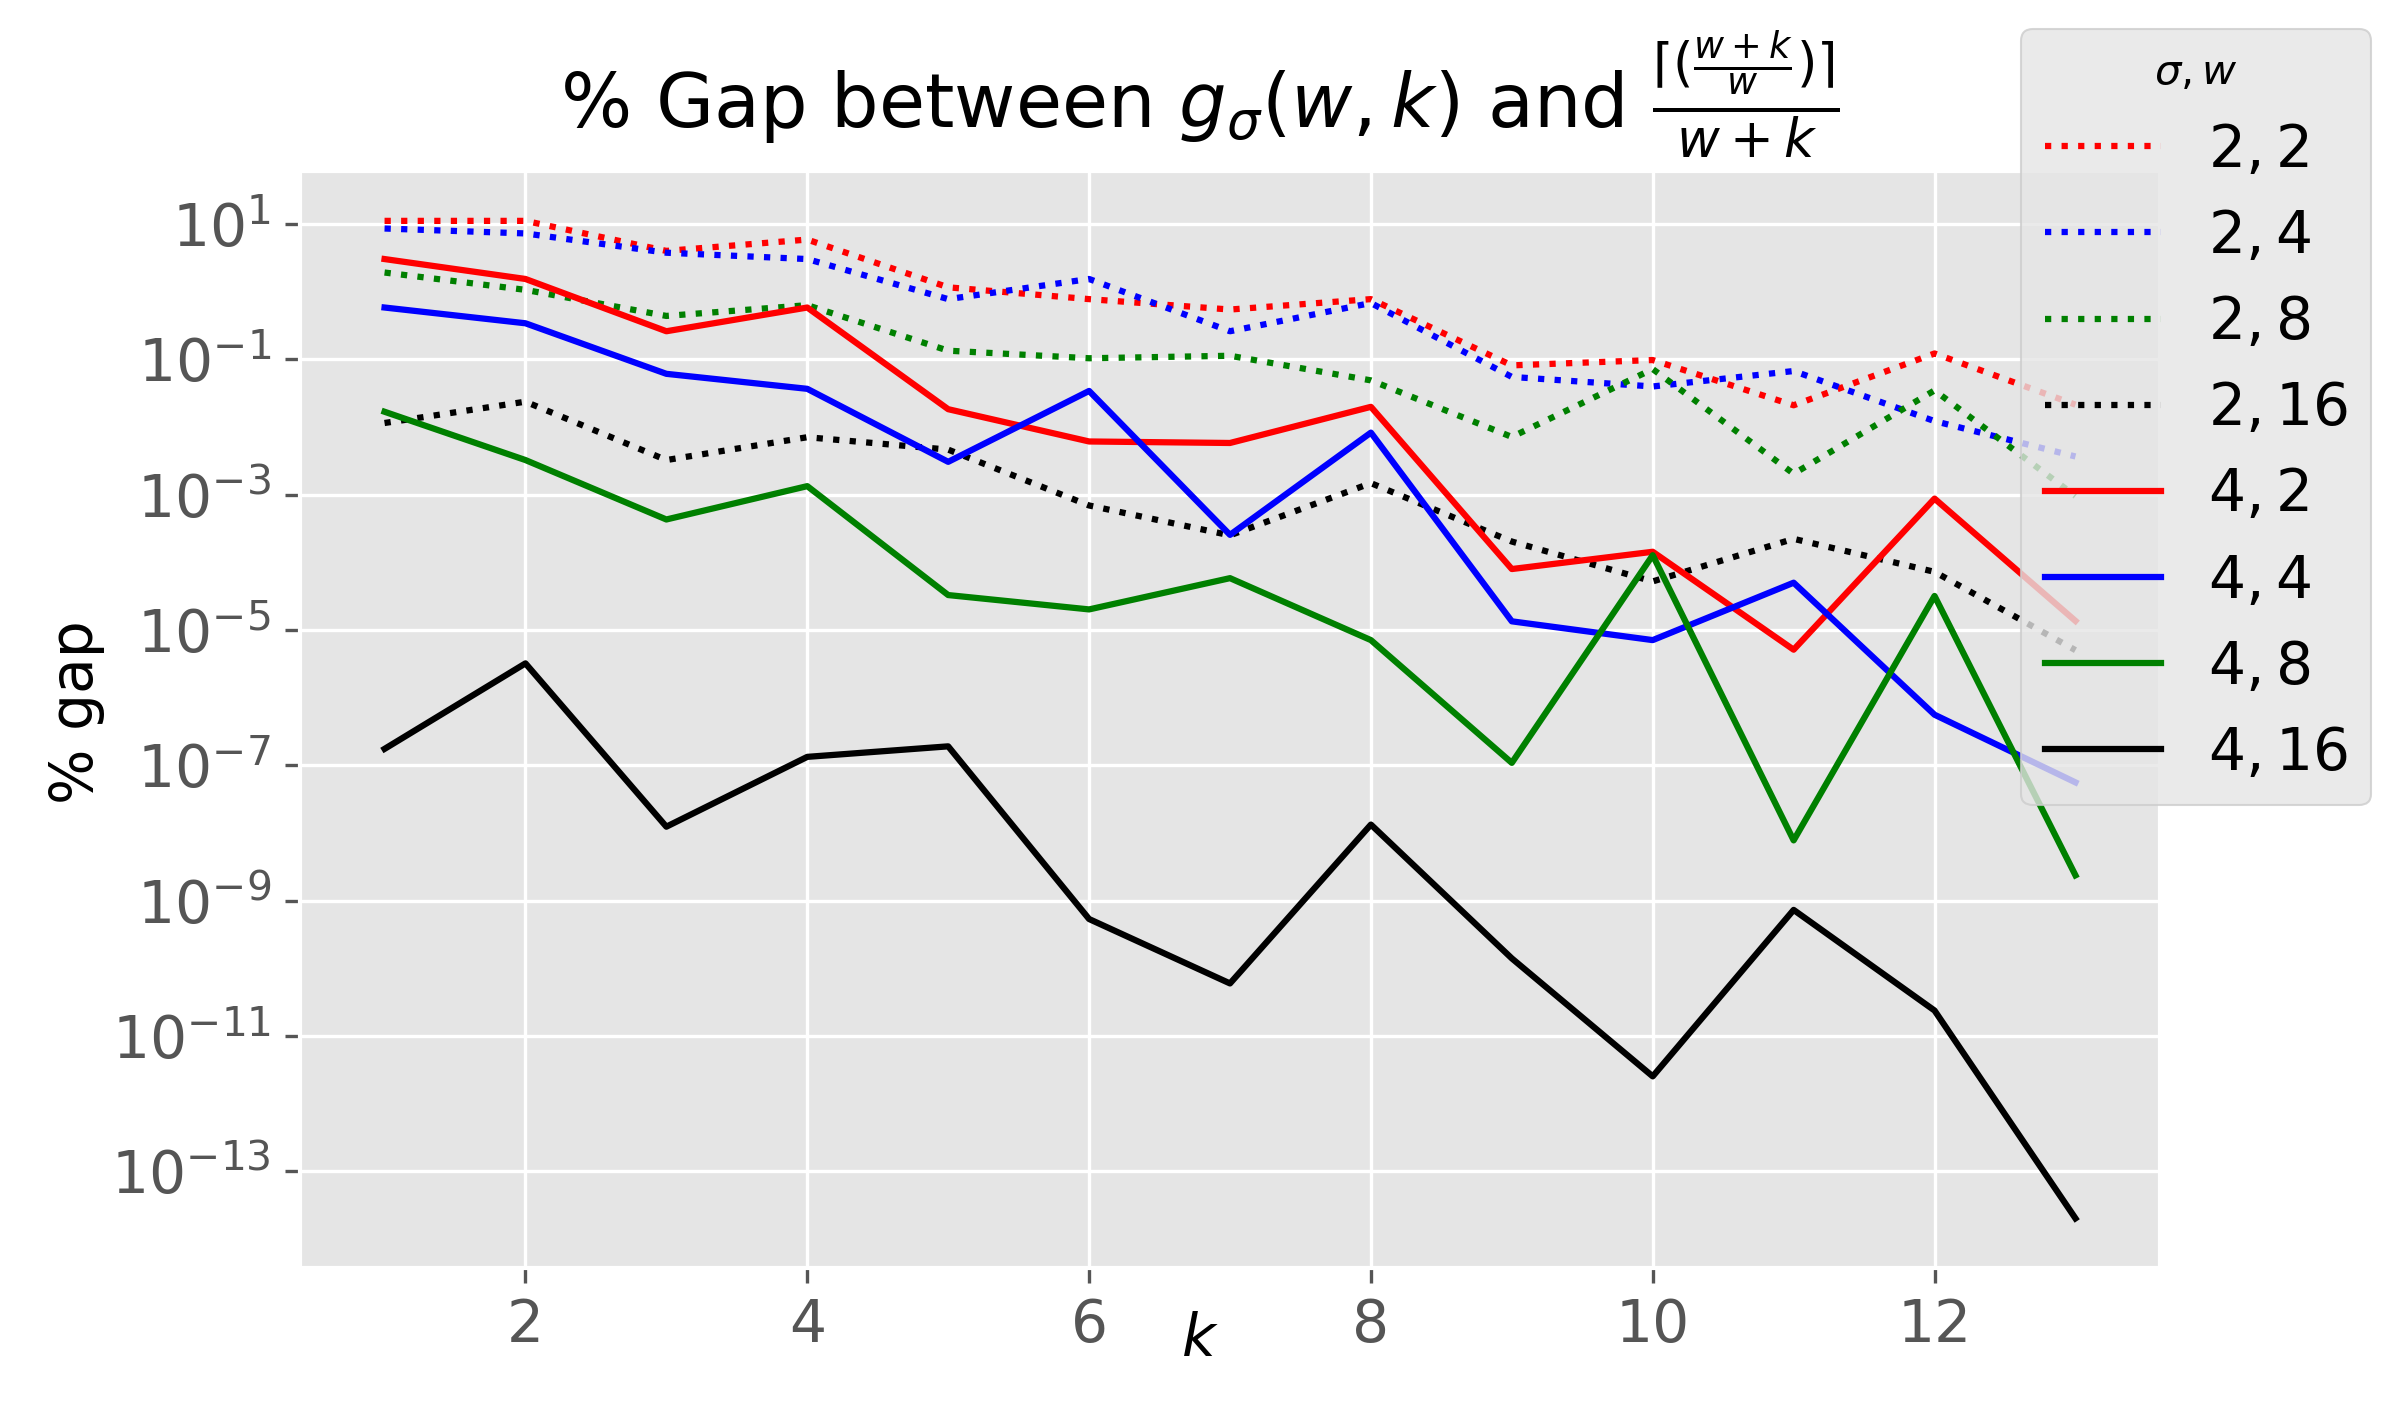
\includegraphics[width=\textwidth]{media/gap-sigma24.png}
\caption{Comparison of $g_\sigma(w, k)$ and ${\ceil*{\frac{w+k}{w}}}/{(w+k)}$ for $\sigma\in\{2,4\}$. The percent gap is calculated as the ratio between $g_\sigma(w, k) - {\ceil*{\frac{w+k}{w}}}/{(w+k)}$ and ${g_\sigma(w,k)}$. While the gap can be as large as 10\% for small parameter values, it quickly decreases with the increase of any of the parameters.}
\label{fig:gap-sigma24}
\end{figure}

For most of our analysis, we examine the behavior of $w,k$ on a binary alphabet, as larger alphabet sizes are infeasible for our ILP on most parameters. We restricted our $(w,k,\sigma)$ parameters to the following three classes in order to ensure that the model was computationally feasible.

\begin{samepage}
\begin{itemize}
    \item Fixed alphabet size $\sigma=2$ (Figure \ref{fig:fwd-bound-sigma2})
    \item Fixed \kmer{} size $k=1$ (Figure \ref{fig:fwd-bound-k1})
    \item Fixed window size $w=2$ (Figure \ref{fig:fwd-bound-w2})
\end{itemize}
\end{samepage}

As can be seen in Figure~\ref{fig:fwd-bound-sigma2}, the ILP was only able to obtain the minimum density for a small set of $w,k$ on a binary alphabet. However, for all ILP solutions when $k\equiv 1\mod w$, the bound $g_2$ was tight. To see how this pattern extended to other alphabet sizes, we fixed $k=1$ and identified optimal solutions for small $w,\sigma$ (Figure~\ref{fig:fwd-bound-k1}). For all of these parameter sets in which our ILP terminated, $g_2$ was tight. 

Finally, we varied $k$ and $\sigma$ with a fixed window size $w=2$ (Figure \ref{fig:fwd-bound-w2}). For all computationally feasible parameters, $g_{2}(2, k)$ was tight for odd $k$ and $g_{2}'(2, k)$  was tight for all $k$. 

\begin{figure}[ht]
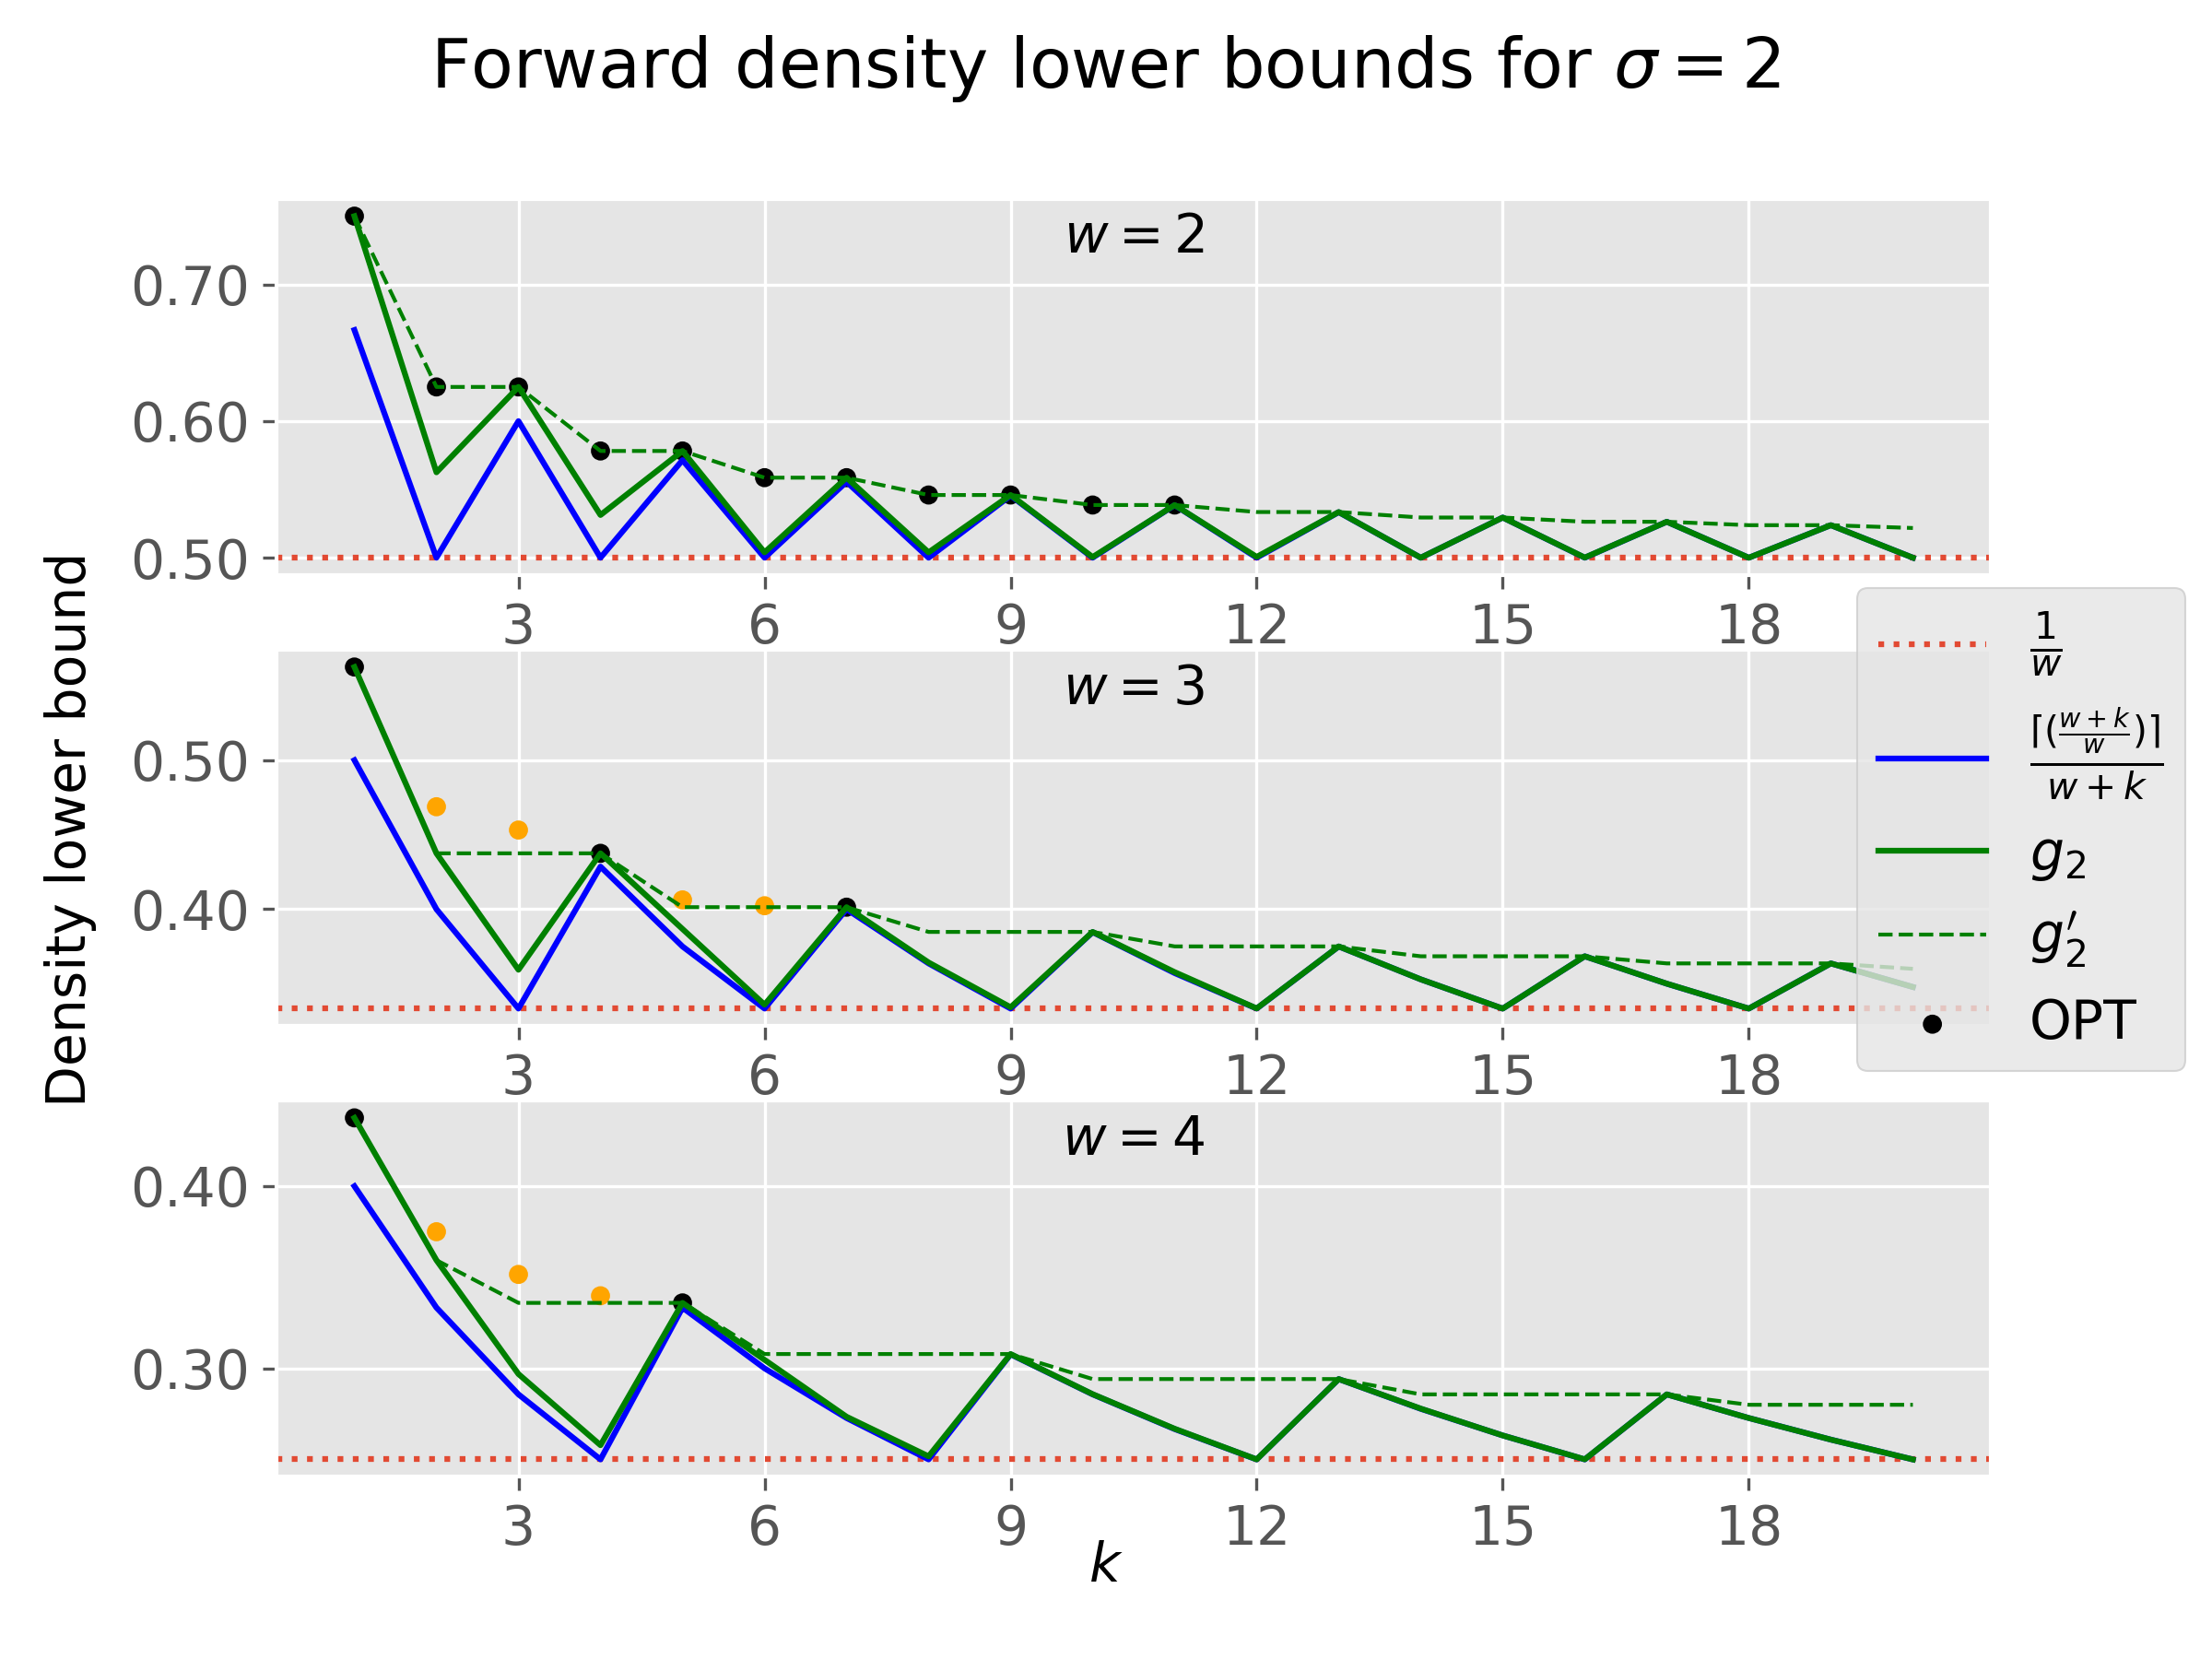
\includegraphics[width=\textwidth]{media/bound-fwd-sigma2.png}
\caption{Comparison of forward scheme bounds for small $w,k$, on a binary alphabet. Minimum densities obtained via the ILP (OPT) are colored black when they match $g'_\sigma$ and orange otherwise.}
\label{fig:fwd-bound-sigma2}
\end{figure}


\begin{figure}[ht]
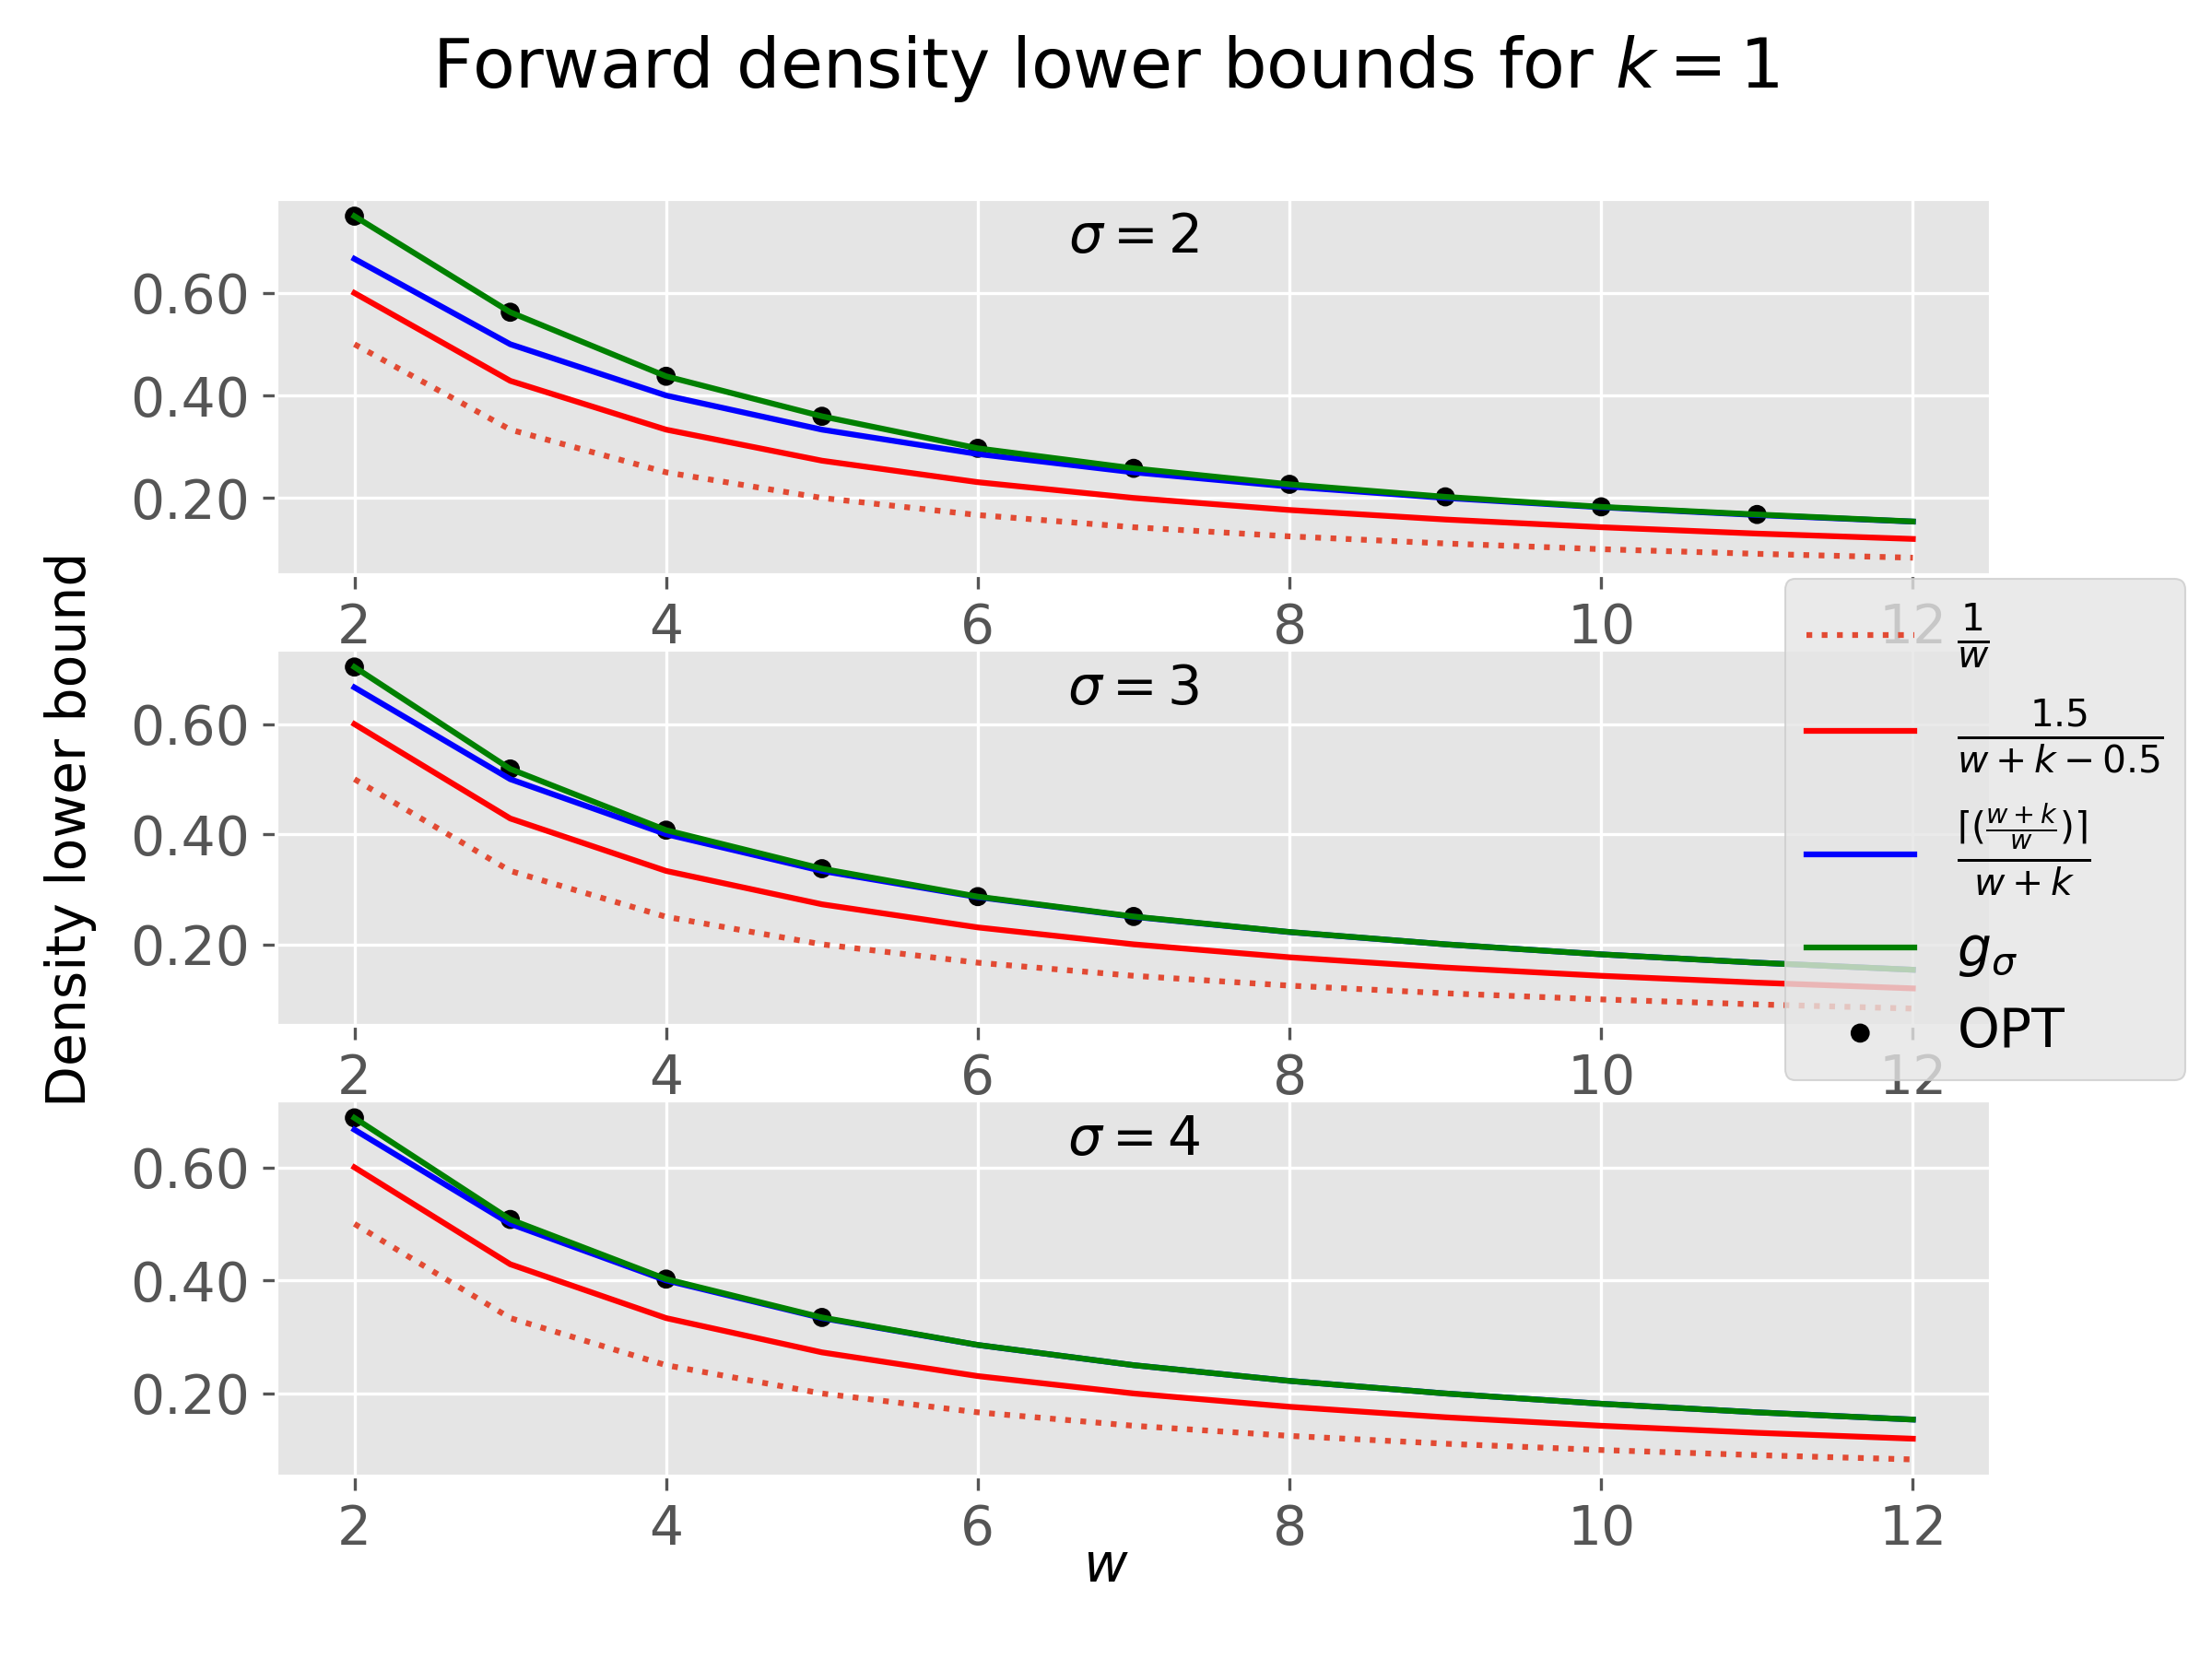
\includegraphics[width=\textwidth]{media/bound-fwd-k1.png}
\caption{Comparison of forward scheme bounds for small $w, \sigma$ with $k=1$. The minimum densities obtained via the ILP (OPT) matched $g_\sigma$ for all tested $w, \sigma$ pairs.}
\label{fig:fwd-bound-k1}
\end{figure}

\begin{figure}[ht]
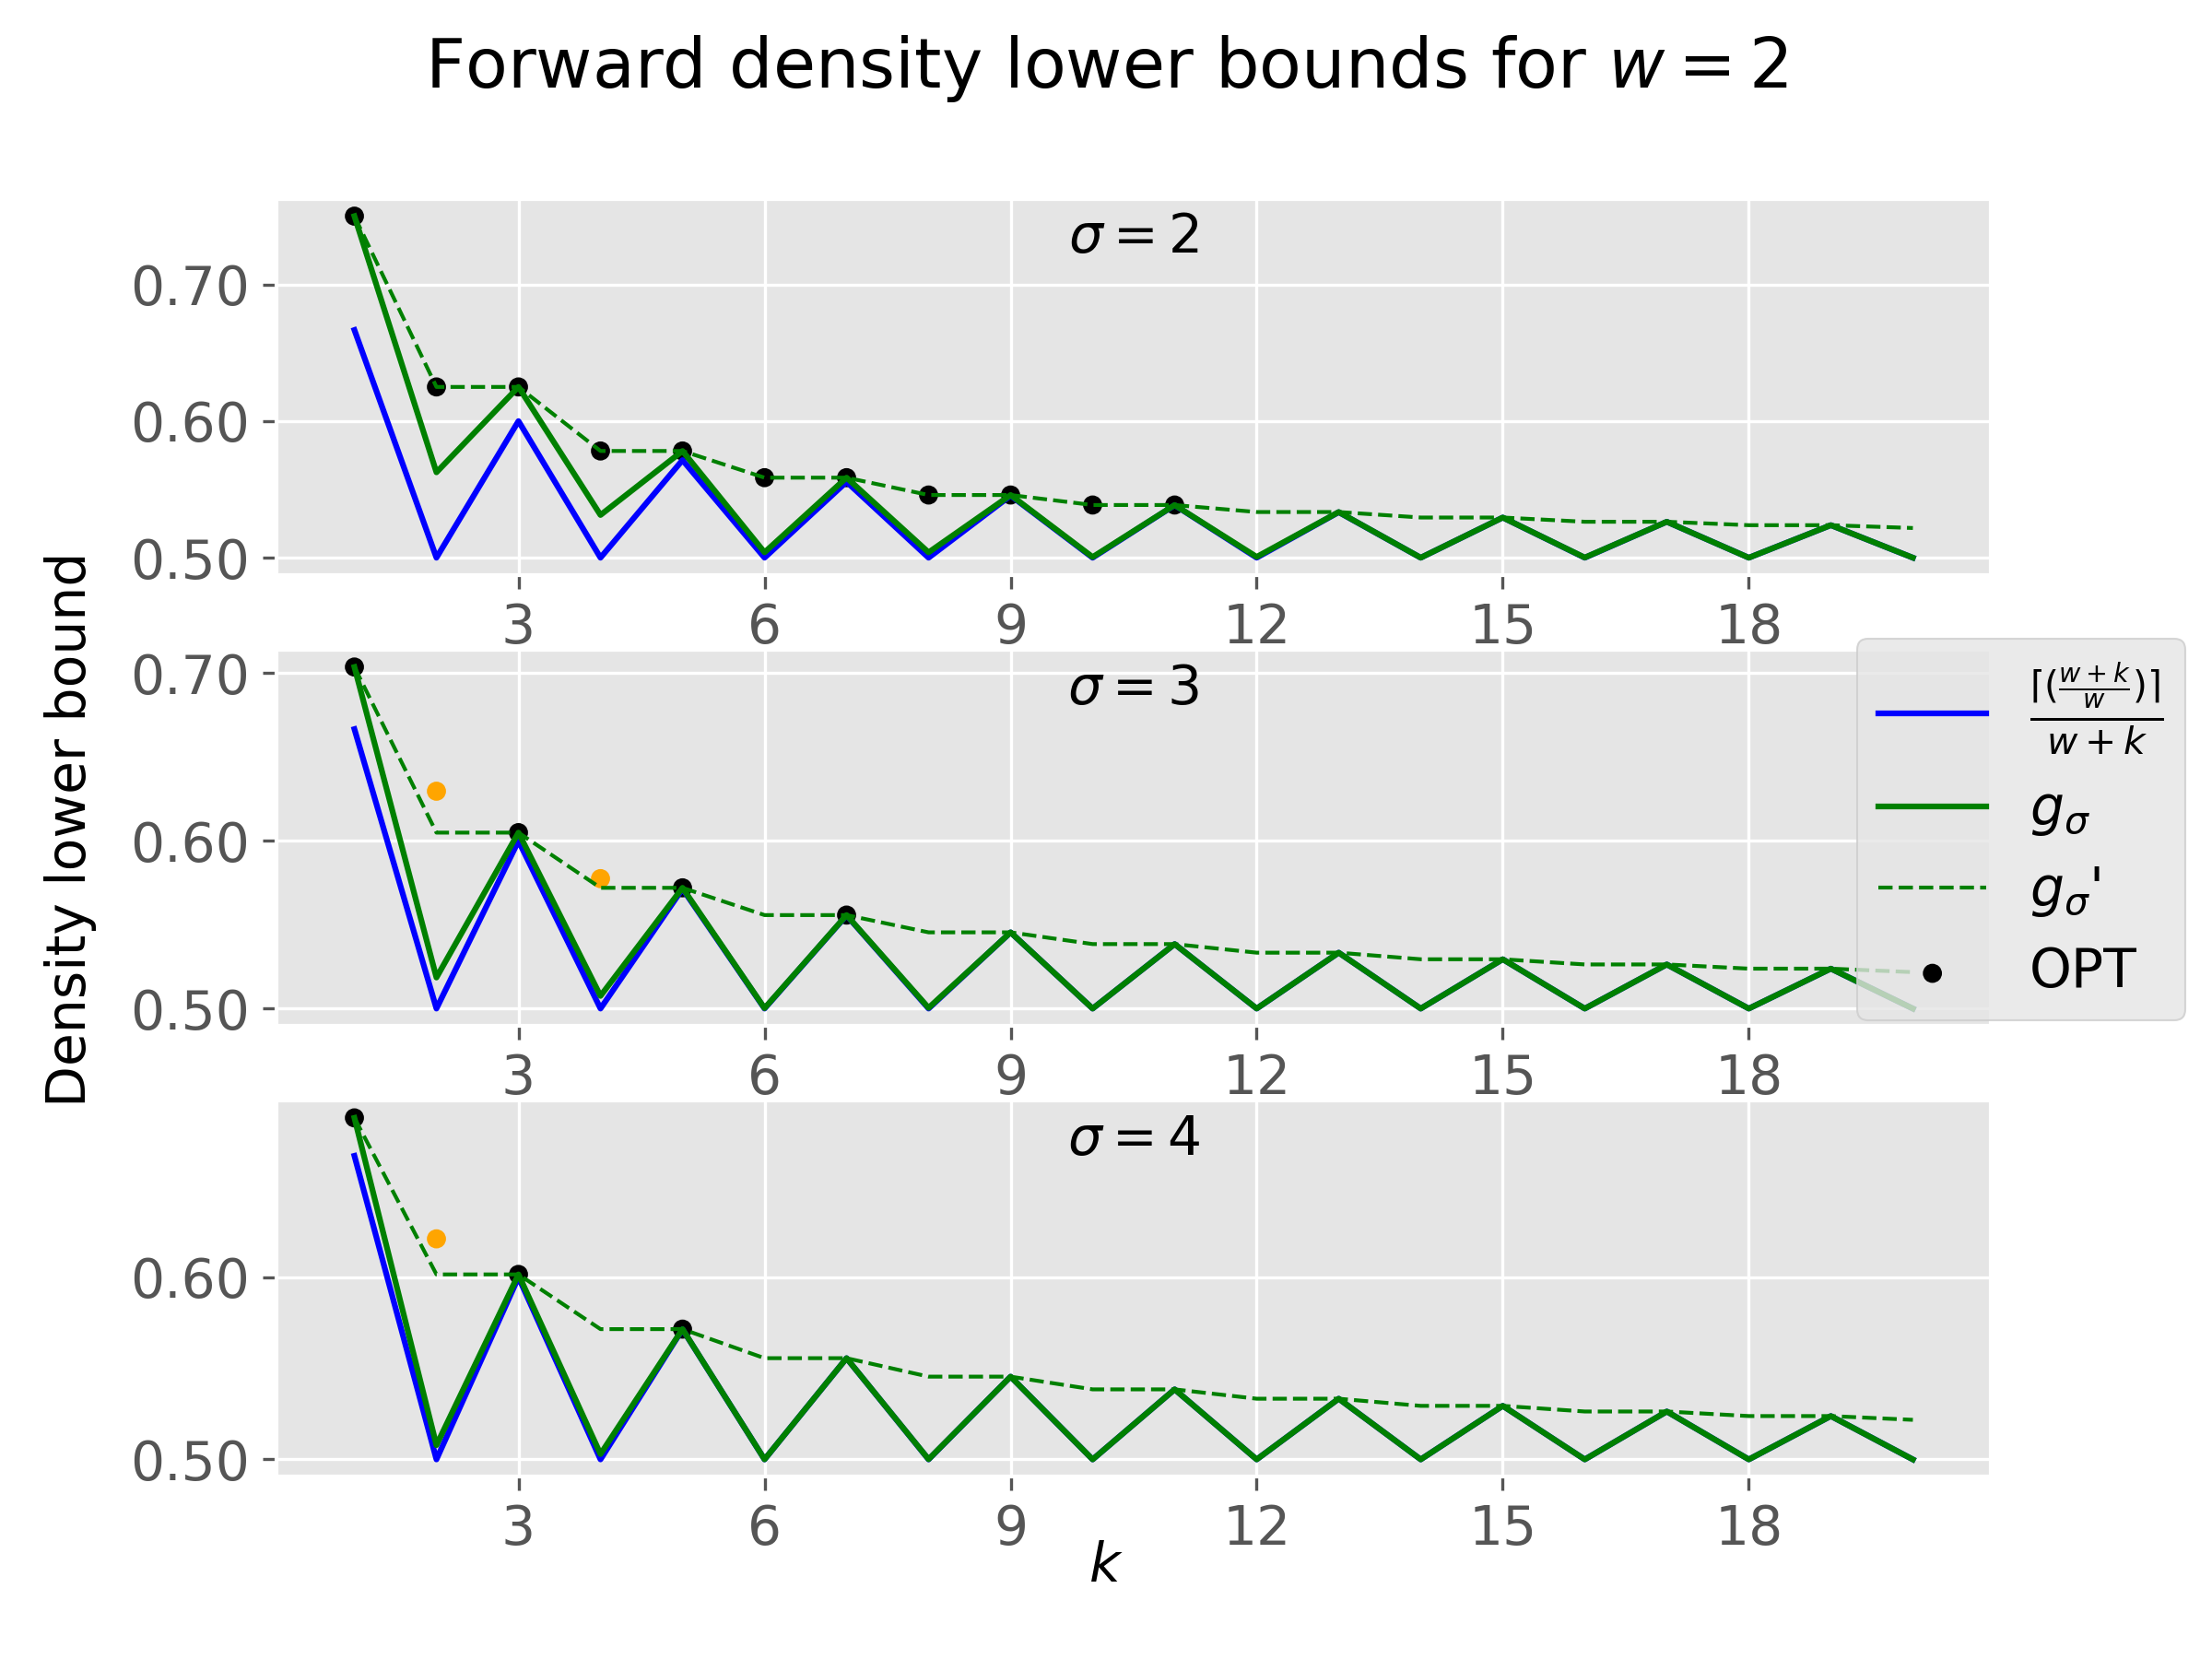
\includegraphics[width=\textwidth]{media/bound-fwd-w2.png}
\caption{Comparison of forward scheme bounds for $w=2$. Minimum densities obtained via the ILP (OPT) are colored black when they match $g'_\sigma$ and orange otherwise.}
\label{fig:fwd-bound-w2}
\end{figure}



\section{Discussion}

By combining the logic used to bound the independence number of de Bruijn graphs with the relationship between universal hitting sets and winnowing scheme densities, we constructed new lower bounds on the density of winnowing schemes which are significantly tighter than previously known bounds. These new lower bounds leverage the well-studied pure cycle partitioning of de Bruijn graphs, providing intuition on how to achieve a minimum density winnowing function in some cases.

Analytically, it is clear that $g_\sigma(w,k)$ is much tighter than previous bounds. However, it was still necessary to determine how tight $g_\sigma(w,k)$ is. To answer this, we obtained minimum density winnowing functions for a subset of small $w, k, \sigma$ through the use of an ILP model. In all cases, $g'_\sigma(w,k)$ was nearly tight, if not completely. For $w=2, \sigma=2$, $g'_\sigma(w,k)$ matched the minimum density for all tested $k\in[11]$. However, for non-binary alphabets, the bound was only tight for odd $k$. Using Corollary \ref{cor:w2-closed}, we arrive at the following conjecture:

\begin{conjecture}
    \label{conj:w2}
For odd $k$, there exists a $(2, k, \sigma)$-local scheme $f$ such that \\$D(f) = \frac{\sigma^{k+2}+\mathcal{N_\sigma}(k+2)}{2\sigma^{k+2}}$.
    
\end{conjecture}

Proving Conjecture~\ref{conj:w2} would be a significant result for both the bioinformatics and graph theory communities, as in addition to an optimal local winnowing scheme, it would yield a result for the independence number of binary de Bruijn graphs as well as all $B_{p,\sigma}$ for prime $p$~\citep{lichiardopol2006independence}. While Conjecture~\ref{conj:w2} only claims that $g_\sigma(w, k)$ is tight for odd $k$, it is known that an independent set in $B_n$ corresponds to a maximum cut in $B_{n-1}$\citep{chvatal1990note} and thus an independent set in $B_{n-1,2}$ of half the size of the independent set in $B_{n, 2}$ can likely be constructed from this maximum cut partitioning.  Therefore, proving Conjecture \ref{conj:w2} would close a long-standing open problem in graph theory in addition to providing an optimal local winnowing scheme for $w=2$. 

In addition to the pattern which led to Conjecture~\ref{conj:w2}, our bound was tight for $k=1$ and the 20 pairs of $w\in[12], \sigma \in \{2, 3, 4\}$ where our ILP identified an optimal solution. We were able to identify a few other $(w,k)$ where our bound was tight for $\sigma=2$: $(3, 4), (3, 7), (3, 10)$, and $(4, 5)$. This leads us to our second conjecture:  
\begin{conjecture}
    \label{conj:k1mw}
For any pair of $w$ and $k$ such that $k\mod w \equiv 1$,  there exists a $(w,k,\sigma)$-forward winnowing function $f$ such that $D(f)=g_\sigma(w, k)$.
\end{conjecture} 
A notable case of Conjecture \ref{conj:k1mw} is $k=1$, as it captures the ``opposite'' boundary of the parameter space relative to Conjecture~\ref{conj:w2} where $w=2$. We hypothesize that solving either one of these cases is the most practical approach to fully characterize the minimum density of winnowing schemes. For example, in order to prove Conjecture~\ref{conj:k1mw}, one would need to come up with a scheme which has has 2 charged edges for each aperiodic necklace of edges, and only 1 charged edge for each of the remaining edge necklaces. 

A natural investigation which follows our proposed lower bound is to determine the gap between $g_\sigma(w,k)$ and current forward scheme densities. Previously, the gap between known densities and lower bound was rather large, making it unclear how much more the density could be reduced. The mod-minimizer scheme recently proposed in \cite{groot2024mod} was proven to be able to achieve density equal to ${\ceil*{\frac{w+k}{w}}}/{(w+k)} + o(\frac{1}{w+k})$ when $k \mod w \equiv 1$ for a sufficiently large alphabet. Since we know due to Lemma \ref{lem:simple-vs-complex} that ${\ceil*{\frac{w+k}{w}}}/{(w+k)}< g_\sigma^\prime(w, k)$,  we have that the gap between existing schemes and known lower bounds is $o(\frac{1}{w+k})$, but only in the case where the alphabet size is much larger than $4$.   

\section{Conclusion}
In this work, we provided a new lower bound for the density of both forward and local winnowing schemes which is orders of magnitude tighter than any existing bounds. The bound incorporates the rich structure of de Bruijn graphs and yields insights as to how an optimal winnowing function would need to be constructed. We used an ILP model to compute minimum densities for a subset of $w, k, \sigma$. By incorporating our lower bound into the model, we were able to generate minimum densities for larger parameter sets and in doing so, we revealed a pattern of our new lower bound being tight for $k\mod w\equiv 1$.

We conclude with two conjectures. Namely, that our provided lower bound $g_\sigma(w, k)$ is tight for $w=2, \sigma=2$, odd $k$ and also for any $w, k, \sigma$ such that $k\mod w\equiv 1$. These conjectures are supported by multiple optimal solutions obtained via an ILP model. We show an equivalence between minimum density $(2, k, \sigma)$-local schemes and the long-standing problem of identifying the independence number of de Bruijn graphs. Proving either of these conjectures would mark a significant milestone in the theory of winnowing schemes, as it would be the first tight lower bound for any nontrivial $(w,k,\sigma)$-forward scheme for a subset of $(w, k, \sigma)$. 


%Bibliography
\bibliography{references}  

\section{Appendix}


\subsection{Additional Proofs}
\begin{lemma}
If $w>1$, then
$$g_\sigma(w, k) > \frac{\ceil*{\frac{w+k}{w}}}{w+k}$$
\end{lemma}

\begin{proof}
\label{proof:simple-vs-complex}
Rewrite the bound given by Corollary \ref{cor:fwd-dens-LB}.
\begin{align*} 
g_\sigma(w,k)&= \sum_{d|w+k}\frac{\mathcal{M}_\sigma(d)(d+(-d \mod w))}{w\sigma^{w+k}}\\
&= \frac{1}{w} + \sum_{d|w+k}\frac{d\mathcal{M}_\sigma(d)(-d \mod w)}{d\sigma^{w+k}}
\end{align*}
We similarly rewrite $\frac{\ceil*{\frac{w+k}{w}}}{w+k}$ to get
\begin{align*} 
\frac{\ceil*{\frac{w+k}{w}}}{w+k}&= \frac{w+k+(-k \mod w)}{w(w+k)}\\
&=\frac{1}{w} + \frac{-k \mod w}{w(w+k)}
\end{align*}
Comparing $$(w+k)\sum_{d|w+k}\frac{d\mathcal{M}_\sigma(d)(-d \mod w)}{d\sigma^{w+k}}~~~~~~~\text{and}~~~~~~~-k \mod w,$$
we see that the left hand side is the average of $\sigma^{w+k}$ values of the form $\frac{(w+k)(-d \mod w)}{d},$ where each value corresponding to some $d|w+k$ is repeated $d\mathcal{M}_\sigma(d)$ times. We can see that
\begin{equation*}
\frac{(w+k)(-d \mod w)}{d} \geq -k \mod w
\end{equation*}
for all $d|w+k.$ To check this, let $m = (w+k)/d,$ so that $-md \equiv -k \mod w.$ Then we have the left and right side respectively 
\begin{align*}
m(-d \mod w)\\ 
-md \mod w
\end{align*} 
These are equivalent modulo $w,$ but the right side must be the least nonnegative residue, whereas the left can be greater. In fact, when $d = 1$ and $w > 1,$ we have the strict inequality 
\begin{equation*}
(w+k)(w-1) >w> -k \mod w
\end{equation*}
Since $1|(w+k)$ for all $w+k,$ this means the average is strictly greater than $-k \mod w$ when $w > 1$. Hence, the corresponding bound given by Corollary \ref{cor:fwd-dens-LB} is also strictly greater than $\frac{\ceil*{\frac{w+k}{w}}}{w+k}$ when $w > 1$.
\end{proof}


\subsection{ILP Models}
\label{appendix:ILP-desc}
\subsubsection{Forward Schemes}

Given a de Bruijn graph $B_{n, \sigma}=(V,E)$, we define our model as follows:
\begin{align}
    \text{maximize} &=~ \sum y~ \\
     \text{such that}\;x_u &\in [w] & \forall u\in V \\\
    y_{(u,v)} &\in \{0, 1\} & \forall (u,v)\in E \\
   y_{u,v} = 1 & \implies  x_u = x_v + 1   &\forall (u,v)\in E\\
   y_{u,v} = 0 & \implies  x_u \leq x_v    &\forall (u,v)\in E
    % x_u ~&\leq~ x_v + 1 + M(1 - y_{u,v}) \\
    % x_u ~&\geq~ x_v + 1 - M(1 - y_{u,v})
\end{align}

% \subsubsection{Local Schemes}

% Let $S$ be a de Bruijn sequence with $|S| = n$, $X = \{x_{u,i}\,|\,u \in V \land 0 \leq i \leq w-1\}, Y = \{y_i\,|\,0 \leq i \leq n-k\}$. Furthermore, let $L = w+k-1$, or the window length, for notation convenience.
% \newline \newline
% Then, we are looking to satisfy
% \begin{align}
%     \min ~~ d ~&=~ \frac{\sum y_i}{n-k+1}~ \\
%     (ILP)~~s.t.~~\text{integer } x_{u,i} ~&\geq~ 0 \\
%     \text{integer } x_{u,i} ~&\leq~ 1 \\
%     \sum\limits_{i=0}^{w-1}x_{u,i} ~&=~ 1 \\
%     \text{integer } y_{u,v} ~&\geq~ 0 \\
%     \text{integer } y_{u,v} ~&\leq~ 1 \\
%     \forall y_m \in Y,~~y_m ~&\leq~ \sum\limits_{i=\max(0,m-w+1)}^{\min(n-L,m)} x_{S[m:m+L),m-i} \\
%     \forall y_m \in Y,~~y_m ~&\geq~ \max\limits_{i \in [\max(0, m-w+1), \min(n-L, m)]}x_{S[m,m+L),m-i}
% \end{align}
%




\end{document}
